\section{The BCS Ground State}
% Logistics
% Final exam is Dec. 16 - 9:30, ANGU 292
% OH on Dec 14/15
% A5 not collected, but posted - do it!

We discuss the 1956 result of Bardeen, Cooper and Schrieffer, who answered the question - what happens to many (as opposed to one, as we studied last lecture) electrons in the presence of attractive interaction?

Today, we go through a historical account of the story. Schrieffer wrote down the wavefunction via intuitition, and then it was shown that this had minimal energy. This is a bit unwieldy and complex, but still interesting. On Wednesday, we discuss the more modern approach to SCs, which also will be more applicable to finite temperature (vs. today's lecture's result, which is only applicable at $T = 0$).

\subsection{Ground State Wavefunction}
We write:
\begin{equation}
    \ket{\psi_G} = \prod_\v{k} \left(u_\v{k} + v_\v{k} c^\dag_{\v{k}\uparrow}c^\dag_{-\v{k}\downarrow}\right)\ket{0}
\end{equation}
%\textcolor{blue}{NOTE - actually equation 10, building on the last lecture}
and then solve the variational problem where $\mu_{\v{k}}, v_\v{k}$ are the variational parameters. We will find that the minimum energy variational state will have lower energy than if we just put all the electrons in the lowest energy states.

For normalization, we have the condition
\begin{equation}\label{eq-ukvknormalization}
    \abs{u_\v{k}}^2 + \abs{v_\v{k}}^2 = 1.
\end{equation}
$\abs{v_\v{k}}^2$ is the probability that the pair $(k\uparrow, -k\downarrow)$ is occupied.

An immediate possible objection - $\ket{\psi_G}$ is a superposition of states with different electron numbers. There are famous physicists who to this day do not accept the wavefunction. To clarify this point, we can write:
\begin{equation}
    \ket{\psi_G} = \sum_N \lambda_N \ket{\psi_N}
\end{equation}
where $\ket{\psi_N}$ is a state with a definite number $N$ of electrons. Bardeen would answer to this objection - this is true, but $\lambda_N$ is very sharply peaked around $N = \bar{N}$. This is a simple calculation:
\begin{equation}
    \bar{N} = \bra{\psi_G}\hat{N}\ket{\psi_G} = \sum_\v{k} 2\abs{v_\v{k}}^2 \sim \Omega
\end{equation}
the last expression follows from the fact that $\abs{v_{\v{k}}}$ are constants of order one, so taking $\sum_{\v{k}} \to \Omega \int d^3k$, we se that the sum scales with volume. Similarly, we can calculate:
\begin{equation}
    \avg{(\hat{N} - \bar{N})^2} = 4\sum_{\v{k}}\abs{u_{\v{k}}}^2\abs{v_{\v{k}}}^2 \sim \Omega
\end{equation}
Therefore:
\begin{equation}
    \frac{\delta N}{\bar{N}} = \frac{\sqrt{(\hat{N} - \bar{N})^2}}{\bar{N}} \sim \frac{\sqrt{\Omega}}{\Omega} \sim \frac{1}{\sqrt{\Omega}} \sim \frac{1}{\sqrt{\bar{N}}}
\end{equation}
Now, since $\bar{N} \sim 10^{22}$, $\delta N \sim \sqrt{\bar{N}} \sim 10^{11}$ so the distribution $P(\lambda_N)$ is sharply peaked:

\begin{figure}[htbp]
    \centering
    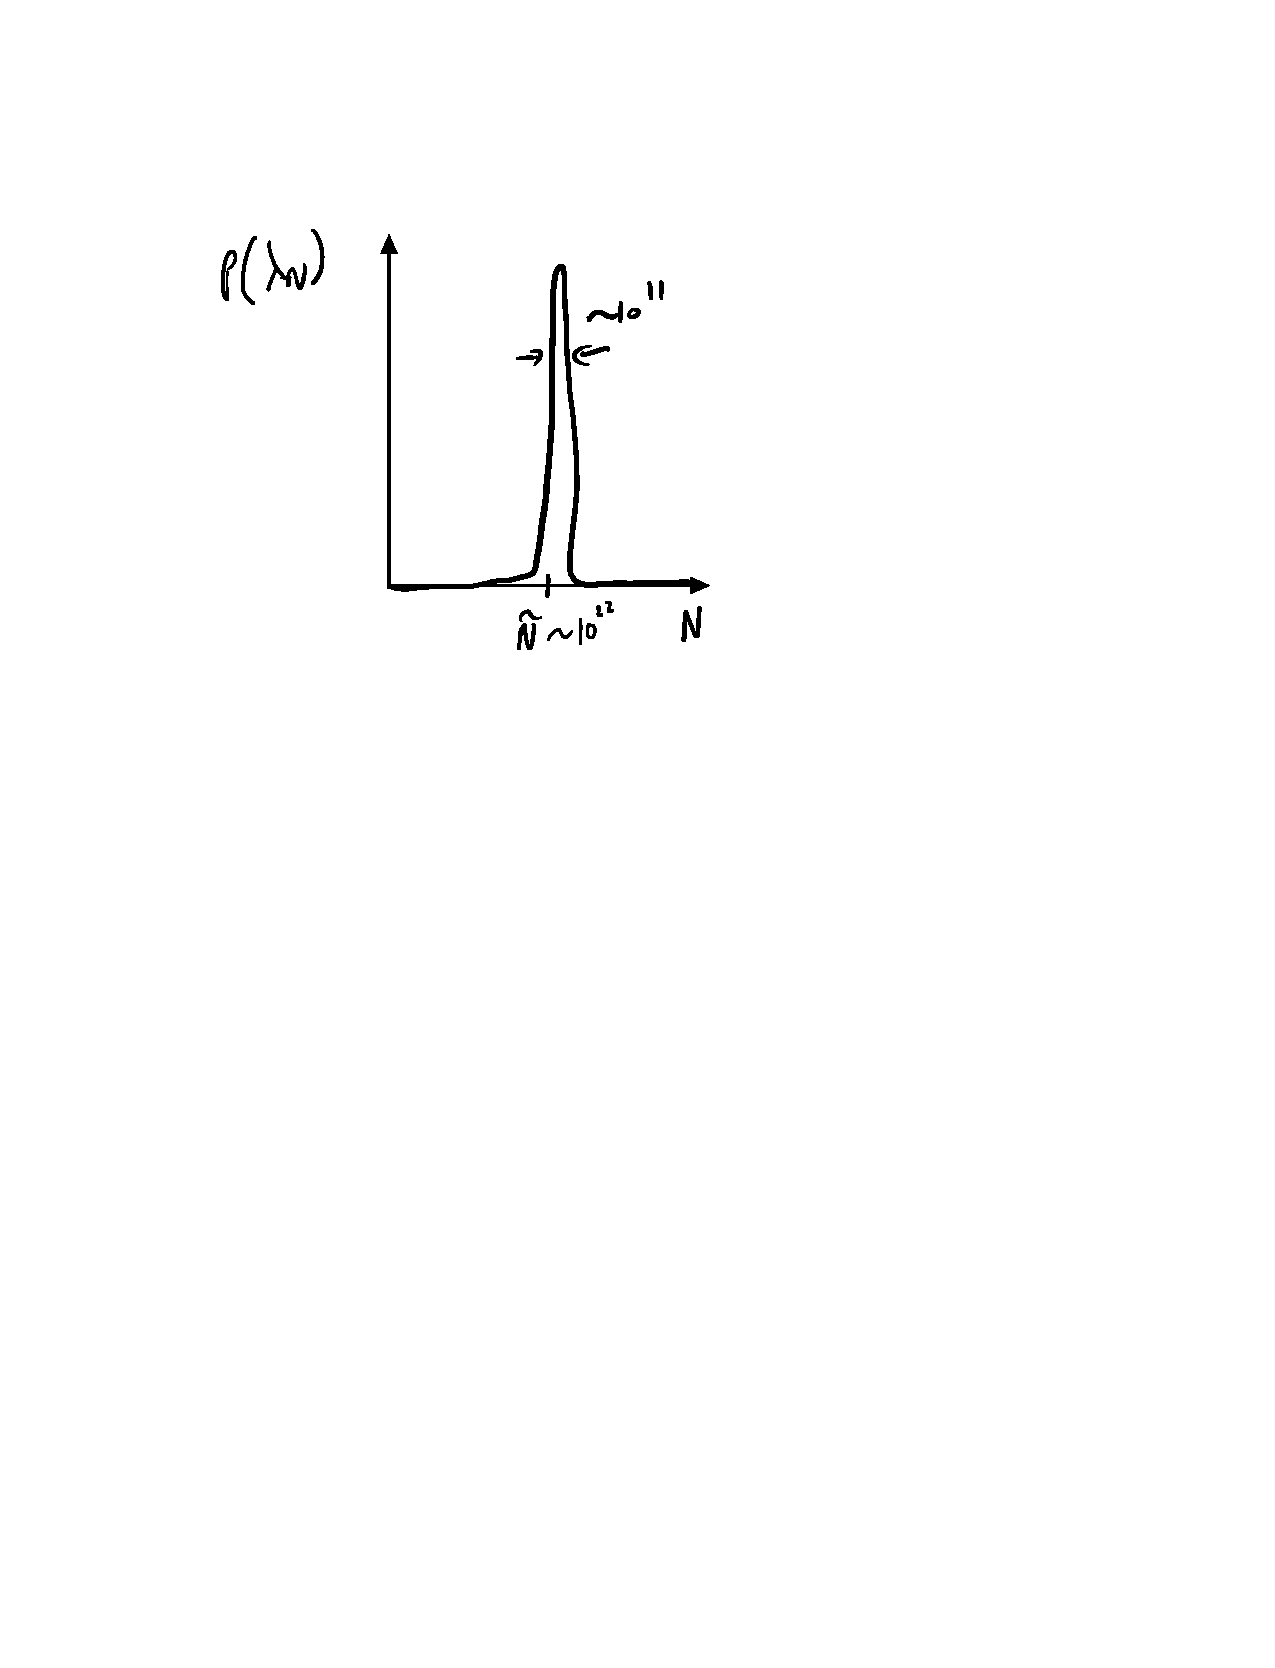
\includegraphics[scale=0.7]{Images/fig-localizedlambdaN.pdf}
    \caption{Plot of $P(\Lambda_N)$ as a function of the electron number $N$. The distribution is sharply peaked around $\bar{N}$.}
    \label{fig-localizedlambdaN}
\end{figure}

So, the BCS wavefunction describes a state with the number of electrons extremely sharply peaked around $\bar{N}$. Note we could calcualte the distribution in principle by expanding out the product and then evaluating the products of $u_{\v{k}}$s and $v_{\v{k}}$s.

\subsection{Calculation of $u_k, v_k$}
We consider the Pairing Hamiltonian, or the BCS Hamiltonian as it is known today. Writing it down, we have:
\begin{equation}
    \hat{H} - \mu \hat{N} = \sum_{\v{k}\sigma}(\e_{\v{k}} - \mu)c^{\dag}_{\v{k}\sigma}c_{\v{k}\sigma} + \sum_{\v{k}\v{l}}V_{\v{k}\v{l}}c^\dag_{\v{k}\uparrow}c^\dag_{-\v{k}l}c_{-\v{l}\downarrow}c_{\v{l}\uparrow}
\end{equation}
The first term is the kinetic energy, the second is the interaction. Where does this come from? We recall the general form of the two body interaction is:
\begin{equation}
    \sum_{\v{kpq}\sigma\sigma'} V_\v{q}c^\dag_{\v{k} - \v{q}\sigma}c^\dag_{\v{p} + \v{q}\sigma'}c_{\v{p}\sigma'}c_{\v{k}\sigma}
\end{equation}
And then motivated by our discussion last class of two electrons on opposite sides of the Fermi sphere having attractive interaction, we enforce $\v{p} = -\v{k}$ and $\v{k} + \v{q} = \v{l}$. This yields the interaction term in the BCS Hamiltonian.

\begin{figure}[htbp]
    \centering
    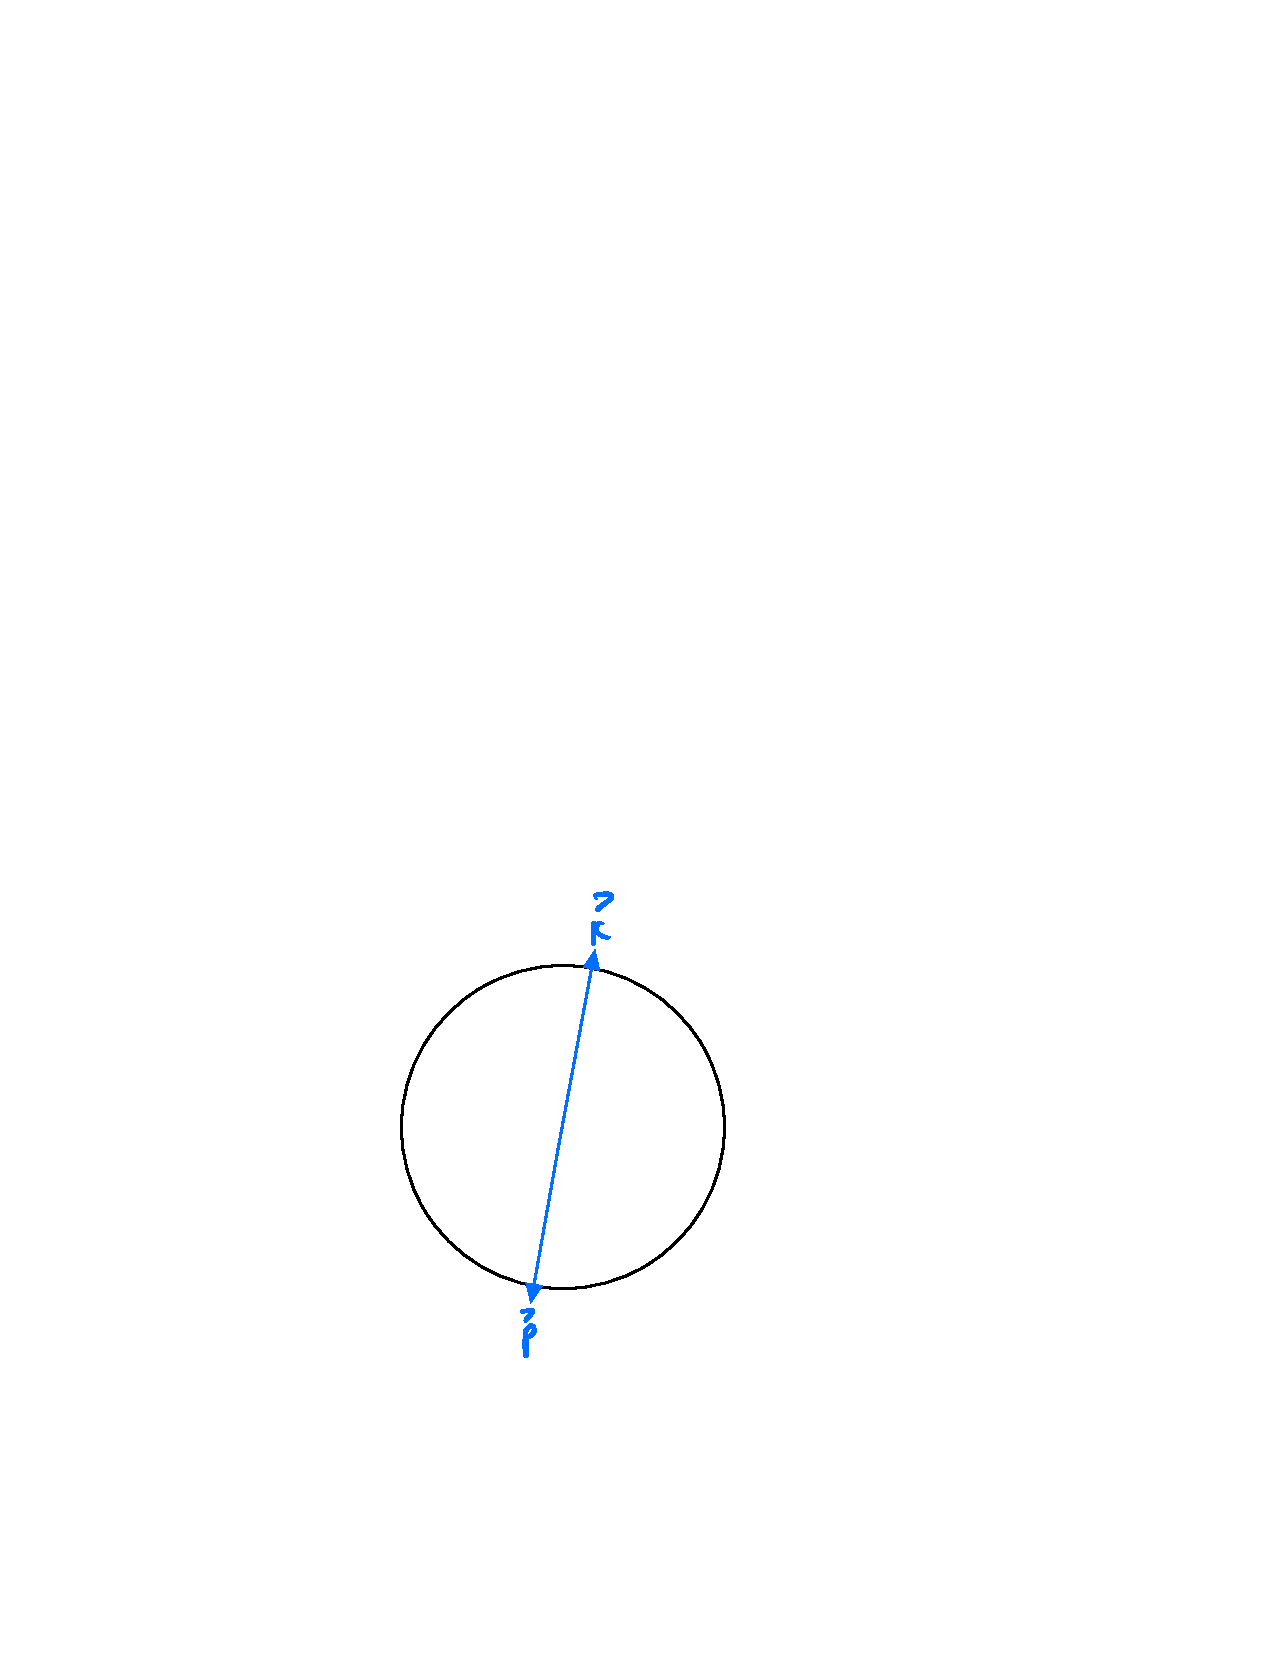
\includegraphics[scale=0.7]{Images/fig-fermisphereopposingelectrons.pdf}
    \caption{We restrict the sum of interactions to be electrons at opposing points above the Fermi sphere.}
    \label{fig-fermisphereopposingelectrons}
\end{figure}

We now calculate the ground state energy. This is another simple, if lengthy calculation:
\begin{equation}
    E_S = \bra{\psi_G}\hat{H} - \mu\hat{N}\ket{\psi_G} = 2\sum_{\v{k}}\xi_{\v{k}}\abs{v_{\v{k}}}^2 + \sum_{\v{k}, \v{l}}V_{\v{k}\v{l}}u_{\v{k}}v_{\v{k}}^* u_{\v{l}}^* v_{\v{l}}
\end{equation}
where $\xi_{\v{k}} = \e_{\v{k}} - \mu$. We minimize this with respect to $u_\v{k}, v_{\v{k}}$. Let as assume that $u_\v{k}, v_\v{k} \in \RR$ (relaxing this assumption does not result in immediately significant changes). An immediate simplification is that $u_\v{k}, v_\v{k}$ are not independent via the normalization condition in Eq. \eqref{eq-ukvknormalization}. So, let us parameterize $u_\v{k} = \sin(\theta_\v{k}), \cos(\theta_{\v{k}})$. We then obtain:
\begin{equation}
    \begin{split}
        E_s &= 2\sum_{\v{k}}\xi_{\v{k}}\cos^2(\theta_\v{k}) + \sum_{\v{k}, \v{l}}V_{\v{k}\v{l}} \cos(\theta_\v{k})\sin(\theta_{\v{k}})\cos(\theta_{\v{l}})\sin(\theta_{\v{l}}) \\ &= \sum_{\v{k}}\xi_{\v{k}}(1 + \cos2\theta_{\v{k}}) + \frac{1}{4}\sum_{\v{k}\v{l}}V_{\v{k}\v{l}}\sin 2\theta_{\v{k}}\sin 2\theta_{\v{l}}
    \end{split}
\end{equation}
Now we minimize (for a given $\v{k}$)
\begin{equation}
    \begin{split}
        0 &= \dpd{E_S}{\theta_{\v{k}}} = -2\xi_{\v{k}}\sin 2\theta_{\v{k}} + \sum_{\v{l}}V_{\v{k}\v{l}}\cos2\theta_{\v{k}}\sin2\theta_{\v{l}}
        \\ \implies \tan 2\theta_{\v{k}} = \frac{\sum_{\v{l}}V_{\v{k}\v{l}}\sin2\theta_{\v{l}}}{2\xi_{\v{k}}}
    \end{split}
\end{equation}
Now, let us define:
\begin{equation}
    \begin{split}
        \Delta_{\v{k}} &= -\sum_{\v{l}}V_{\v{k}\v{l}}u_{\v{l}}v_{\v{l}} = -\frac{1}{2}\sum_{\v{l}}V_{\v{k}\v{l}}\sin2\theta_{\v{l}}
        \\ E_{\v{k}} &= \sqrt{\xi_{\v{k}}^2 + \Delta_\v{k}^2}
    \end{split}
\end{equation}
So with this, we have:
\begin{equation}
    \tan2\theta_{\v{k}} = -\frac{\Delta_{\v{k}\v{l}}}{\xi_\v{k}}
\end{equation}
Now, writing:
\begin{equation}
    \begin{split}
        2u_{\v{k}}v_{\v{k}} &= \sin2\theta_{\v{k}} = \frac{1}{\sqrt{1 + \tan^{-2}2\theta_{\v{k}}}} = \frac{\Delta_{\v{k}}}{E_{\v{k}}}
        \\ v_{\v{k}}^2 - u_{\v{k}}^2 &= \cos2\theta_{\v{k}} = \frac{-1}{\sqrt{2 + \tan^22\theta_{\v{k}}}} = -\frac{\eta_{\v{k}}}{E_{\v{k}}}
    \end{split}
\end{equation}
We can now solve:
\begin{equation}
    \begin{split}
        v_{\v{k}}^2 &= \frac{1}{2}\left(1 - \frac{\xi_{\v{k}}}{E_{\v{k}}}\right)
        \\ u_{\v{k}}^2 &= \frac{1}{2}\left(1 + \frac{\xi_{\v{k}}}{E_{\v{k}}}\right)
    \end{split}
\end{equation}
The last step is to calculate $\Delta_{\v{k}}$ (from its definition) so we can make sense of $E_{\v{k}}$. We find:
\begin{equation}
    \Delta_{\v{k}} =-\frac{1}{2}\sum_{\v{l}} \frac{\Delta_{\v{l}}}{E_{\v{l}}}V_{\v{k}\v{l}} = -\frac{1}{2}\sum_{\v{l}}\frac{\Delta_{\v{l}}}{\sqrt{\xi_{\v{l}}^2 + \Delta_{\v{l}}^2}}V_{\v{k}\v{l}}
\end{equation}
this is now a self-consistent equation for $\Delta$. To solve, we use Cooper's Ansatz:
\begin{equation}
    V_{\v{k}\v{l}} = \begin{cases}
        -V & \text{if $\abs{\xi_{\v{k}}}, \abs{\xi_{\v{l}}} \leq \hbar \omega_c$}
        \\ 0 & \text{otherwise}
    \end{cases}
\end{equation}
So then:
\begin{equation}
    \Delta_{\v{k}} = \begin{cases}
        \Delta & \text{when $\abs{\xi_{\v{k}}} \leq \hbar\omega_c$}
        \\ 0 & \text{otherwise}
    \end{cases}
\end{equation}
And so we obtain the equation:
\begin{equation}
    \Delta = \frac{1}{2}V\sum_{\v{l}}' \frac{\Delta}{\sqrt{\Delta^2 + \xi_{\v{l}}^2}}
\end{equation}
the trivial solution is $\Delta = 0$. If $\Delta \neq 0$, then we can divide out by $\Delta$ on both sides, and obtain:
\begin{equation}
    \frac{2}{V} = \sum_{\v{l}}' \frac{1}{\sqrt{\Delta^2 + \xi_{\v{l}}^2}} = \int_{-\hbar\omega_c}^{\hbar\omega_c} d\xi \frac{N(\xi)}{\sqrt{\xi^2 + \Delta^2}} \approx N(0)\int_{-\hbar\omega_c}^{\hbar\omega_c} \frac{d\xi}{\sqrt{\xi^2 + \Delta^2}} = 2N(0)\arcsinh(\frac{\hbar\omega_c}{\Delta})
\end{equation}
Inverting this to find $\Delta$, we find:
\begin{equation}
    \Delta = \frac{\hbar\omega_c}{\sinh(1/VN(0))}
\end{equation}
this starts to look like the Cooper problem. At weak coupling of $VN(0) \ll 1$, the argument of $\sinh$ is large and we can approximate it as an exponential:
\begin{equation}
    \Delta \to 2\hbar \omega_C e^{-1/VN(0)}
\end{equation}
A few remarks on the physics behind this. This is a non-perturbative result, like Cooper instability. If you expand in powers of $V$, the expansion will fail as there is an essential singularity at $V = 0$. We also note that a non-trivial solution exists for any $V$ attractive. So, the state exists self-consistently!

Let us now plot $v_\v{k}^2$ given this result.

\begin{figure}[htbp]
    \centering
    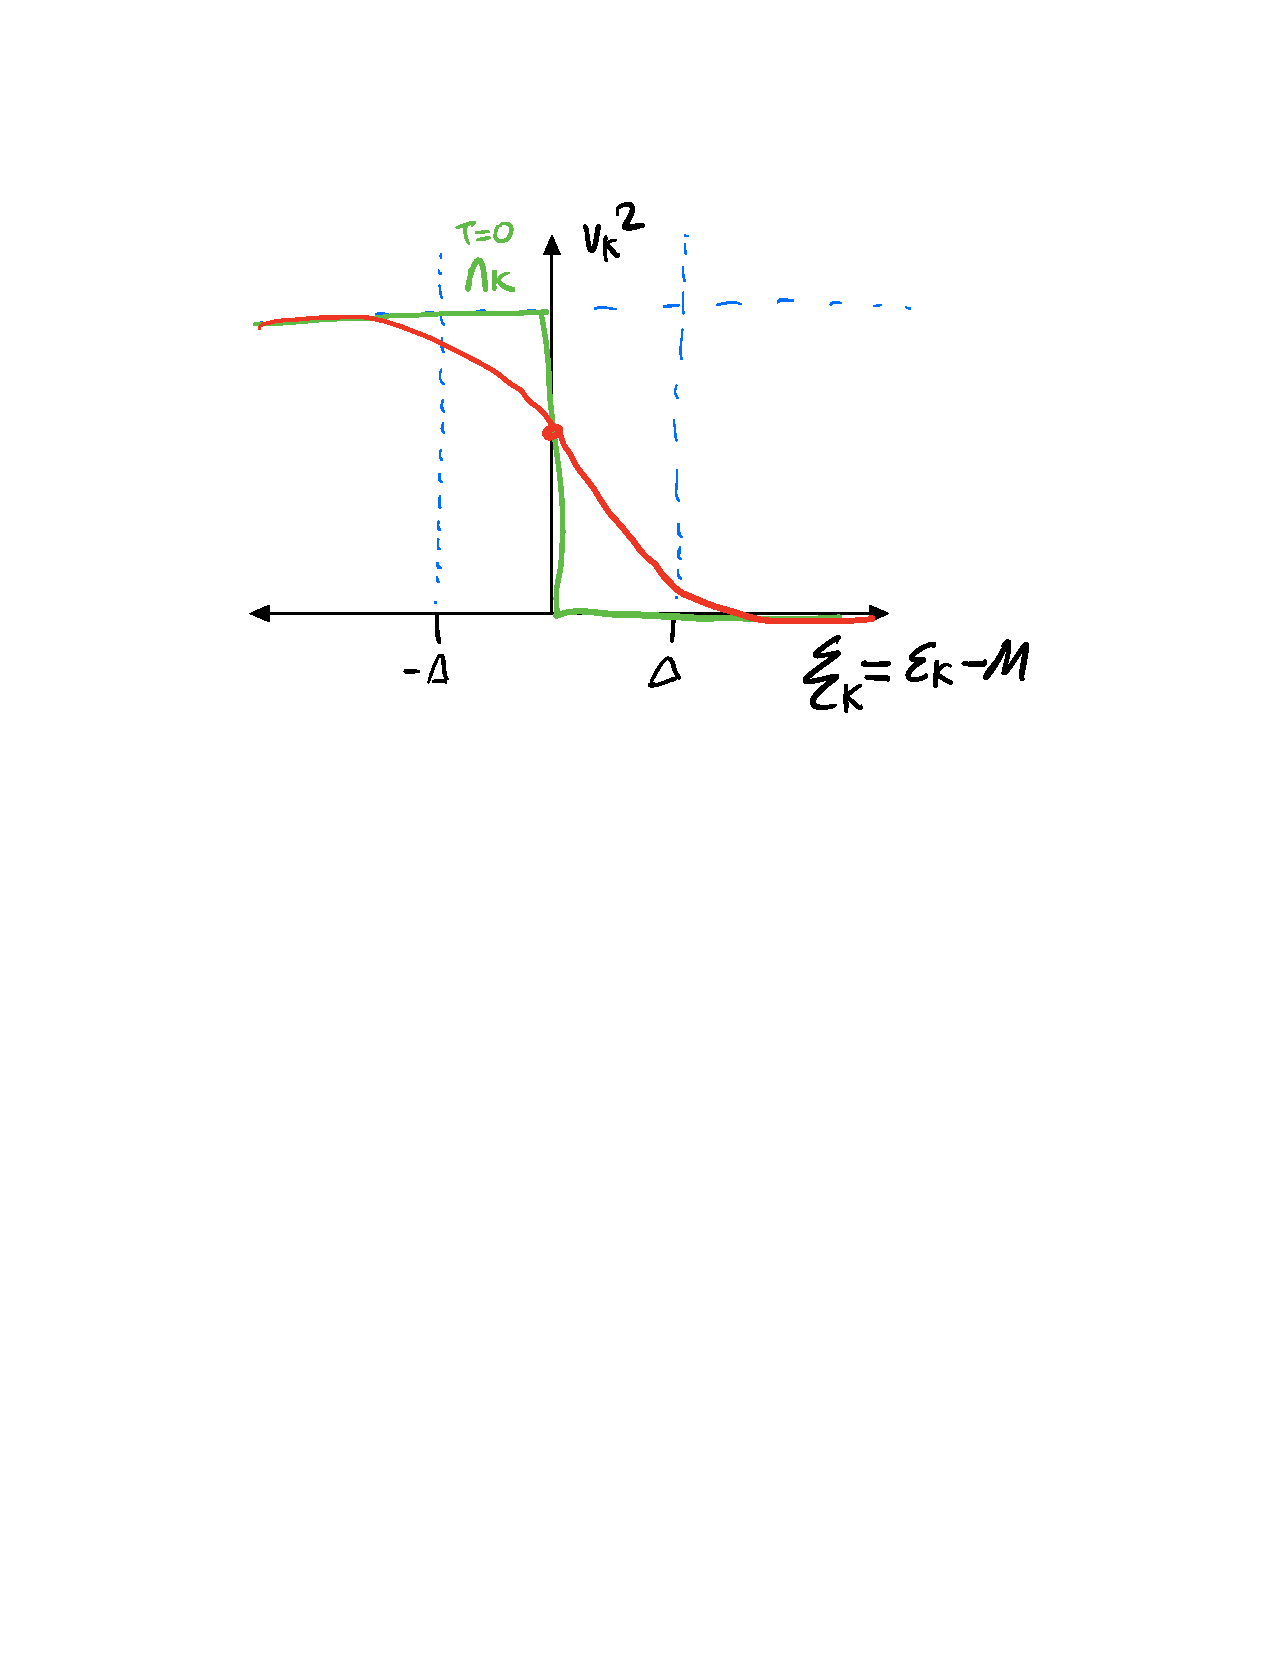
\includegraphics[]{Images/fig-vksquareplotbcs.pdf}
    \caption{Plot of $v_\v{k}^2$ vs $\xi_\v{k}$, with the $T = 0$ Fermi function plotted for comparison.}
    \label{fig-vksquareplotbcs}
\end{figure}

When $\Delta \neq 0$, we have a ``paired state'', different from the filled Fermi sphere.

\subsection{BCS Condensation Energy}
Finally, we show that this paired state has lower energy than the Fermi sphere:
\begin{equation}
    \begin{split}
        E_s &= \bra{\psi_G}\hat{H} - \mu\hat{N}\ket{\psi_G}
        \\ &= \sum_{\v{k}}\left(\xi_{\v{k}} - \frac{\xi_{\v{k}}^2}{E_k}\right) - \frac{\Delta^2}{V}
    \end{split}
\end{equation}
compare this with the Fermi sphere energy:
\begin{equation}
    E_n = \bra{\psi_G}\hat{H} - \mu\hat{N}\ket{\psi_G}_{\Delta = 0} = 2\sum_{\abs{\v{k}} < k_F} \xi_{\v{k}}
\end{equation}
and so:
\begin{equation}
    \boxed{\delta E = E_s - E_n = -\frac{1}{2}N(0)\Delta^2}
\end{equation}
note the minus sign - the condensation energy is negative $\delta E \leq 0$, anytime $\Delta$ is nonzero. This implies that $\ket{\Psi_G}$ is a stable state. It has energy lower than the Fermi sphere.

If you read the original BCS paper, they go onto discuss the physical implications of this. But unfortunately because the calculation was at zero temperature, the calculations are lengthy and roundabout. Instead, next time we show the modern treatment of this problem via a standard mean-field theory, and do a finite temperature calculation. From those results we will be able to readily evaluate the properties of a superconducting state.